\section{Protokol WebRTC}\label{webRTC}

V této části práce vychází převážně z publikace
\href{https://webrtcforthecurious.com/}{WebRTC For The Curious: Go beyond the
    APIs} \parencite{WebRTCForTheCurious}.

\gls{webrtc} je protokol, který umožňuje vytvoření bezpečného obousměrného
spojení mezi dvěma klienty pro přeposílání audia, videa a libovolných dat v
reálném čase. Toto spojení může být \gls{p2p}, ale data mohou být přeposílaná i
přes server, jak je popsáno v části \ref{connecting}. Je využíváno koncové
šifrování, anglicky \gls{e2ee}, což zaručuje, že server nemůže číst data, pokud
jsou přes něj přeposílaná~\parencite{WebRTCForTheCurious}.

\gls{webrtc} spojení je složeno ze \textit{stop} (\textit{tracks}) a
\textit{datových kanálů} (\textit{data channels}). Stopa může být buď audio, či
video \parencite{MDN-WebRTC-MediaStreamTrack}. Tyto stopy mohou být přiřazeny do
tzv. \textit{streamů} (stream je často složen ze dvou stop -- např. audia z
mikrofonu a~videa z~kamery)~\parencite{MDN-WebRTC-MediaStream}. Datové kanály se
pak používají k přenosu libovolných dat
\parencite{WebRTCORG-GettingStarted-DataChannels}.

\gls{api} protokolu \gls{webrtc} je specifikováno jen v~JavaScriptu. Existují
však i implementace \gls{webrtc}
(např.~\href{https://github.com/pion/webrtc}{Pion} či
\href{https://github.com/webrtc-rs/webrtc}{WebRTC.rs}) v jiných jazycích
\parencite{WebRTCForTheCurious,GitHub-Pion-WebRTC,GitHub-WebRTCRS-WebRTC}.

Protokol \gls{webrtc} se skládá z mnoha komponentů a využívá ke svému fungování
mnoha jiných protokolů \parencite{WebRTCForTheCurious}. V této části si
jednotlivé komponenty rozebereme a~popíšeme, k čemu slouží.

\subsection{Spojování}\label{connecting}

Tradiční aplikace často používají model klient-server, ve kterém má server
fixovanou známou IP adresu, již může klient využít pro komunikaci. Ve
\gls{webrtc} tomu ale tak není, neboť protokol je \gls{p2p}. Oba klienti jsou
tedy zodpovědní za vytvoření obousměrného spojení, což může být složité. Má to
ale své vyhody jako menší zpoždění. Vývojář se zároveň nemusí starat o žádné
servery \parencite{WebRTCForTheCurious}.

Pro vytvoření spojení se používá protokolu \gls{ice}. Protokol \gls{ice} slouží
k nalezení nejlepšího způsobu, jak vytvořit spojení mezi dvěma klienty. Každý
klient zveřejní své tzv. \textit{\gls{ice} kandidáty}, což jsou v podstatě IP
adresy a~porty, které je možno využít pro komunikaci s ním (více v části
\ref{ice})~\parencite{WebRTCForTheCurious}. V této části se zabýváme jen
samotným výběrem těchto kandidátů; jak si klienti předají informace o
kandidátech je rozebráno v sekci \ref{signalling}.

\subsubsection{NAT}\label{nat}

\begin{figure}[H]
    \centering
    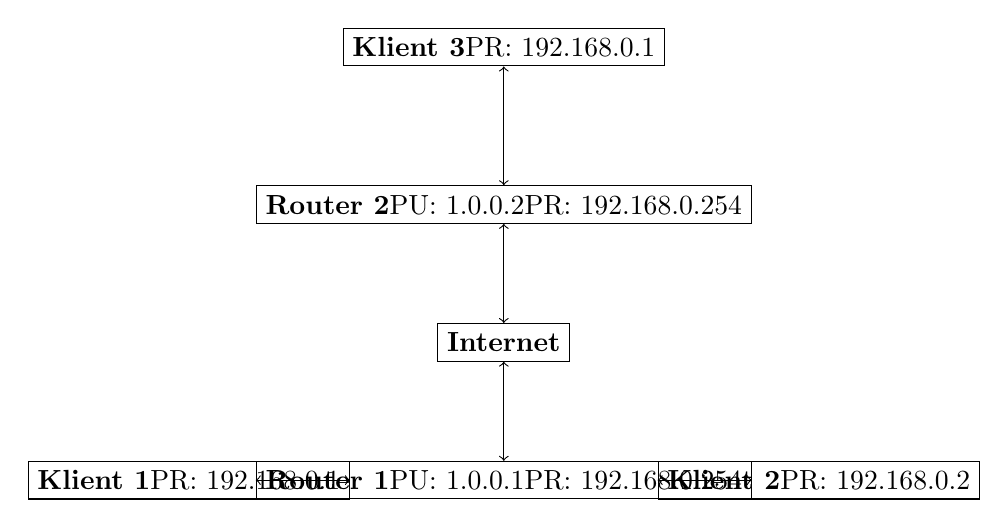
\begin{tikzpicture}
        \node[draw] (client3) at (0,3.75) {\textbf{Klient 3}\\PR: 192.168.0.1};
        \node[draw] (router2) at (0,1.75) {
            \textbf{Router 2}\\
            PU: 1.0.0.2\\
            PR: 192.168.0.254
        };

        \node[draw] (internet) at (0,0) {\textbf{Internet}};

        \node[draw] (router1) at (0,-1.75) {
            \textbf{Router 1}\\
            PU: 1.0.0.1\\
            PR: 192.168.0.254
        };
        \node[draw] (client1) at (-4,-1.75) {\textbf{Klient 1}\\PR: 192.168.0.1};
        \node[draw] (client2) at (4,-1.75) {\textbf{Klient 2}\\PR: 192.168.0.2};

        \draw[<->] (client1) -- (router1);
        \draw[<->] (client2) -- (router1);
        \draw[<->] (router1) -- (internet);

        \draw[<->] (internet) -- (router2);
        \draw[<->] (router2) -- (client3);
    \end{tikzpicture}
    \caption{NAT (\publicPrivateIP)}
    \label{natFig}
\end{figure}

Kvůli nedostatku IPv4 adres je nutno reprezentovat několik zařízení v podsíti
routeru jednou veřejnou IP adresou \parencite{Medium-NATWHyWeNeedIt}. Využívá se
k tomu metody \gls{nat}, která vytváří mapování mezi veřejnou IP
adresou\footnote{Pro zjednodušení předpokládáme statické veřejné IP adresy.} a
portem a privátní IP adresou a portem v podsíti routeru
\parencite{WebRTCForTheCurious}.

Na obrázku \ref{natFig} vidíme situaci, ve které je snadné pro klienta 1 poslat
paket klientovi 2, neboť jsou ve stejné podsíti. Ale pokud by klient 3 chtěl
poslat paket klientovi za routerem~2, je nutné využít veřejných IP adres
routerů. Ty ale klienti nemusí znát. Zároveň je nutné, aby router věděl, na jaký
z klientů paket přeposlat \parencite{WebRTCForTheCurious}.

Jednou z možností mapování je \textit{port forwarding}, jde o statické
namapování předem definovaného portu na privátní IP adresu a port v podsiti
routeru. Router 2 by mohl mít vytvořené takové mapování, že přijde-li paket na
adresu \mintinline{text}{1.0.0.2:80} (tedy na port \mintinline{text}{80} na
routeru 2), router 2 ho přesměruje na adresu \mintinline{text}{192.168.0.1:90}
(port \mintinline{text}{90} na klientovi 3). Pošle-li klient 3 paket mimo podsíť
routeru 2, bude přeposlán routerem přes port \mintinline{text}{80} (příjemce
bude tedy vidět \mintinline{text}{1.0.0.2:80} jako zdrojovou adresu). Toto
mapování je vhodné pro případy, kdy chceme, aby dané zařízení za routerem bylo
dostupné na IP adrese routeru na pevně daném portu
\parencite{G2-WhatIsPortForwarding}.

Mapování ale nemusí být pevné a může existovat jen dočasně. Pošle-li klient 1
paket na~\mintinline{text}{1.0.0.2:80} (port \mintinline{text}{80} na routeru
2), vybere router 1 nějaký port \mintinline{text}{P}, vytvoří mapování
a~přepošle paket z tohoto portu (příjemce bude tedy vidět
\mintinline{text}{1.0.0.1:P} jako zdrojovou adresu). Když následně klient 3
pošle paket na~\mintinline{text}{1.0.0.1:P} (port \mintinline{text}{P} na
routeru~1), router 1 rozpozná dle portu, že má paket zpět přeposlat na
\mintinline{text}{192.168.0.1:80} (klienta 1, který posláním svého paketu
mapování vytvořil). Toto mapování může ale v budoucnosti zaniknout\footnote{Jak
    dlouho je mapování funkční závisí na mnoha faktorech. Např. pokud je použit
    protokol \gls{tcp}, mapování se ruší explicitně.}. Tento typ mapování je
nejčastější pro běžná zařízení \parencite{WebRTCForTheCurious}.

\subsubsection{STUN}\label{stun}

\begin{figure}[H]
    \centering
    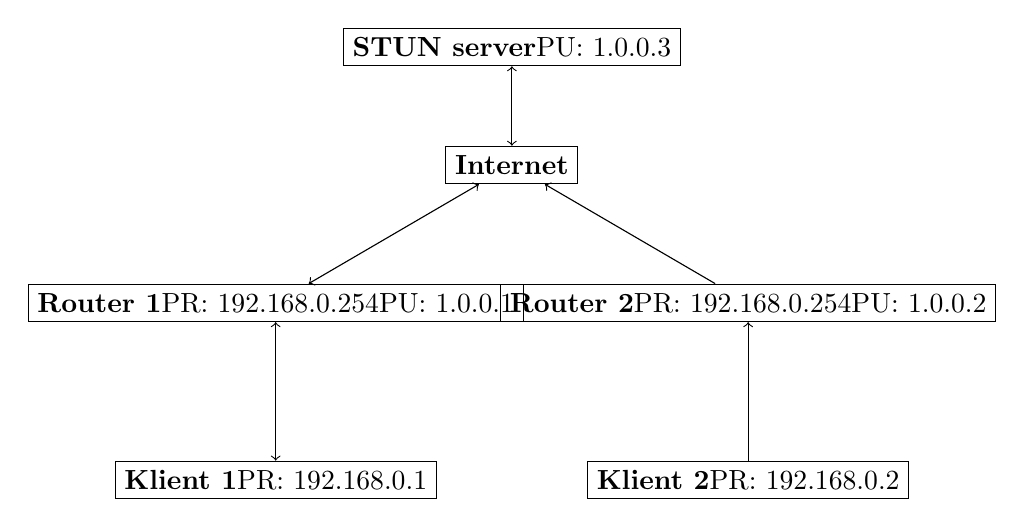
\begin{tikzpicture}
        \node[draw] (stunServer) at (0,1.5) {\textbf{STUN server}\\PU: 1.0.0.3};

        \node[draw] (internet) at (0,0) {\textbf{Internet}};

        \node[draw] (router1) at (-3,-1.75) {
            \textbf{Router 1}\\
            PR: 192.168.0.254\\
            PU: 1.0.0.1
        };
        \node[draw] (client2) at (3,-4) {\textbf{Klient 2}\\PR: 192.168.0.2};

        \node[draw] (router2) at (3,-1.75) {
            \textbf{Router 2}\\
            PR: 192.168.0.254\\
            PU: 1.0.0.2
        };
        \node[draw] (client1) at (-3,-4) {\textbf{Klient 1}\\PR: 192.168.0.1};

        \draw[<->] (client1) -- (router1);
        \draw[<->] (router1) -- (internet);
        \draw[<-] (internet) -- (router2);
        \draw[<-] (router2) -- (client2);

        \draw[<->] (internet) -- (stunServer);
    \end{tikzpicture}
    \caption{STUN (\publicPrivateIP)}
    \label{stunFig}
\end{figure}

\gls{nat} sice umožňuje vytvořit mapování mezi veřejnou IP adresou a portem a IP
adresou a portem v podsíti, ale klienti v podsíti neví, jaká je veřejná IP
adresa routeru (obzvlášť pokud je dynamická), a pokud není použit port
forwarding, neví ani, jaký port bude využit pro přeposílání paketů. \gls{stun}
je protokol, který nám umožňuje tato omezení překonat
\parencite{WebRTCForTheCurious}.

V síti, která je vidět na obrázku \ref{stunFig}, klient 1 pošle
\textit{\gls{stun} Binding Request} na~\mintinline{text}{1.0.0.3} (na~\gls{stun}
server, který má známou statickou veřejnou IP adresu). Router 1 využije metody
\gls{nat} pro vytvoření mapování na určitém portu \mintinline{text}{P}.
\gls{stun} server vidí, že paket přišel z adresy \mintinline{text}{1.0.0.1:P},
tuto informací pomocí \textit{\gls{stun} Binding Response} pošle zpět
na~\mintinline{text}{1.0.0.1:P} (router 1). Protože bylo na routeru 1 vytvořeno
mapování, router 1 ví, že pokud přijde paket na port \mintinline{text}{P}, má
jej přeposlat na IP adresu \mintinline{text}{192.168.0.1} (klientovi 1), ten
poté ze~\gls{stun} Binding Response může vyčíst, jaká je jeho veřejná IP adresa
(někdy také \textit{Mapped Address} či \textit{Server Reflexive Candidate}).
V~podstatě se jedná o automatické dynamické port
forwardování~\parencite{WebRTCForTheCurious}.

Bohužel Mapped Address vůbec nemusí být užitečná, pokud je použito \gls{nat}
mapování typu \textit{Address Dependent}, což znamená, že router 1 přijímá na
daném mapování pakety pouze z IP adresy \mintinline{text}{1.0.0.3} (ze
\gls{stun} serveru)\footnote{Address Dependent mapování lze často také nalézt
    pod pojmem \textit{Symmetric} \gls{nat}. Tento pojem je ale nepřesný, neboť
    reálné \gls{nat} často nelze snadno klasifikovat do kategorií
    \parencite{IETF-RFC4787}.}. \gls{stun} naštěstí umožňuje zjištění typu \gls{nat}
mapování, takže klient předem ví, jestli ho bude možné kontaktovat
\parencite{WebRTCForTheCurious}.

\subsubsection{TURN}\label{turn}

\begin{figure}[H]
    \centering
    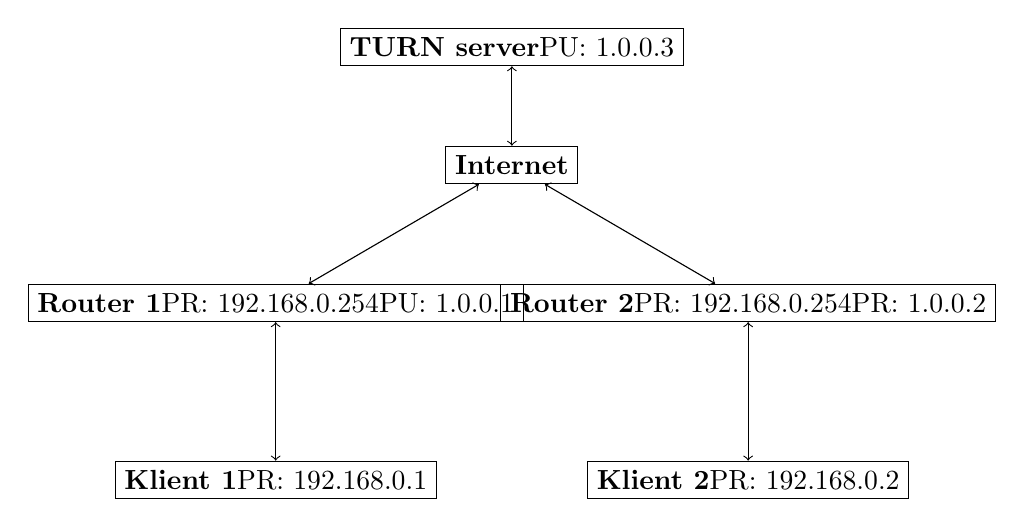
\begin{tikzpicture}
        \node[draw] (turnServer) at (0,1.5) {\textbf{TURN server}\\PU: 1.0.0.3};
        \node[draw] (internet) at (0,0) {\textbf{Internet}};

        \node[draw] (router1) at (-3,-1.75) {
            \textbf{Router 1}\\
            PR: 192.168.0.254\\
            PU: 1.0.0.1
        };
        \node[draw] (client1) at (-3,-4) {\textbf{Klient 1}\\PR: 192.168.0.1};

        \node[draw] (router2) at (3,-1.75) {
            \textbf{Router 2}\\
            PR: 192.168.0.254\\
            PR: 1.0.0.2
        };
        \node[draw] (client2) at (3,-4) {\textbf{Klient 2}\\PR: 192.168.0.2};

        \draw[<->] (client1) -- (router1);
        \draw[<->] (router1) -- (internet);
        \draw[<->] (turnServer) -- (internet);
        \draw[<->] (internet) -- (router2);
        \draw[<->] (router2) -- (client2);
    \end{tikzpicture}
    \caption{TURN (\publicPrivateIP)}
    \label{turnFig}
\end{figure}

\gls{turn} je metoda, která umožňuje vytvořit spojení i v případě, že je
\gls{nat} mapování Address Dependent, či pokud je klient za jiným druhem
restriktivního firewallu. \gls{turn} lze také využít, přeje-li si klient, aby
druhý klient neznal jeho IP adresu \parencite{WebRTCForTheCurious}.

\gls{turn} server funguje jako proxy (prostředník), přes které jsou přeposílána
data. Přeje-li si klient 1 na obrázku \ref{turnFig} využít \gls{turn} server,
musí nejdříve vytvořit tzv. \textit{alokaci}, která je následně využita k
přeposílání dat. Aby alokaci klient 1 vytvořil, musí serveru poskytnout
uživatelské jméno, heslo, protokol (může být \gls{udp} nebo \gls{tcp}) a
port~\parencite{WebRTCForTheCurious}.

Podaří-li se alokaci vytvořit, odpověď \gls{turn} serveru obsahuje podobně jako
u \gls{stun} Mapped Address (v našem případě \mintinline{text}{1.0.0.1:P1}),
\textit{Lifetime} (což je doba, po kterou bude alokace aktivní), \textit{Relayed
    Address} (v našem případě \mintinline{text}{1.0.0.3:P2}, což je adresa, kterou
klient 1 předá ostatním klientům). Pokud jsou na Relayed Adresu
(\mintinline{text}{1.0.0.3:P2}) poslány pakety, budou \gls{turn} serverem
přesměrovány na Mapped Adresu (adresu, ze které byla vytvořena alokace) --
\mintinline{text}{1.0.0.1:P1} (tedy router 1). Ten následně přepošle pakety na
klienta 1 na základě mapování, které bylo vytvořeno při vytváření
alokace~\parencite{WebRTCForTheCurious}.

Nyní musí klient 2 poslat \gls{turn} serveru \gls{stun} Binding Request a
klientovi 1 sdělit svou veřejnou adresu. Klient 1 pak může klientovi 2 povolit,
aby na danou alokaci posílal pakety \parencite{WebRTCForTheCurious}.

Klient 1 může posílat na~\gls{turn} server \textit{Send Indication}, která
obsahuje data, které se mají přeposlat klientovi 2
\parencite{WebRTCForTheCurious}.

Posílá-li se velké množství paketů, může být nevýhodné, aby každý z nich
obsahoval IP adresu a port. Je tedy možné vytvořit tzv. \textit{kanál}
(\textit{Channel}), mající své \textit{ID kanálu} (\textit{Channel ID}). Klient
pak kanál používá v paketech místo IP adresy a portu. Paket je poté na
\gls{turn} serveru upraven a IP adresa a port dodány
\parencite{WebRTCForTheCurious}.

Vzhledem k tomu, že alokace jsou časově omezeny, klient může poslat
\textit{Refresh} request, který by měl prodloužit lifetime dané alokace
\parencite{WebRTCForTheCurious}.

\subsubsection{ICE}\label{ice}

\glsxtrfull{ice} je protokol, který najde všechny páry adres a portů, které je
možné využít pro spojení dvou klientů. Tyto páry se nazývají \textit{páry
    kandidátů}. Může se jednat o privátní adresy v rámci podsítě routeru, Mapped
Adresy (získané ze \gls{stun} serveru), či Relayed Adresy (získané z \gls{turn}
serveru). Klienti komunikují pomocí \textit{\gls{ice} ping paketů}, které
umožňují ověřit funkčnost spojení \parencite{WebRTCForTheCurious}.

\gls{ice} klient je buď \textit{controlling}, nebo \textit{controlled}.
Controlling klient je ten, který vybere vhodný pár kandidátů. Obvykle je
controlling klient ten, který zahájil spojování~\parencite{WebRTCForTheCurious}.

Nabízí-li každá strana 2 kandidáty, existují pak 4 páry kandidátů. Klienti
využijí \gls{ice} ping pakety, aby ověřili, které páry jsou funkční. Ty páry, u
kterých došlo k výměně dat, jsou pak označeny za \textit{validní kandidáty}.
Controlling klient následně vybere jeden z validních párů a označí ho za
\textit{nominovaný pár}. Klienti se pak znovu pokusí o obousměrnou komunikaci
pomocí tohoto páru, a je-li úspěšná, stává se z daného párů \textit{vybraný pár
    kandidátů} \parencite{WebRTCForTheCurious}.

Dojde-li po vytvoření spojení k potížím (např. vyprší \gls{nat} mapování nebo
selže \gls{turn} server), celý proces začne znovu
\parencite{WebRTCForTheCurious}.

\subsubsection{Způsobí přechod na IPv6 zánik ICE a STUN?}

\gls{nat} původně vzniklo jako způsob řešení nedostatku IPv4 adres, ale za léta
svého vývoje se jejich význam rozšířil, neboť zároveň poskytují jednu z vrstev
zabezpečení \parencite{Quora-WillIPv6KillSTUNAndICE}.

Přestože postupný přechod na IPv6 je nevyhnutelný, je nepravděpodobné, že by
technologie jako \gls{nat} zmizely. Je tak smysluplné předpokládat, že
technologie jako \gls{ice} a \gls{stun} rovněž zůstanou relevantní
\parencite{Quora-WillIPv6KillSTUNAndICE}.

\subsection{Přenos audio a videa}

\gls{webrtc} umožňuje posílat neomezené množství audio a~video stop, které buď
mohou být nezávislé, nebo mohou být součástí streamu. Typickým příkladem je
uživatel, který v~jednom streamu posílá audio stopu ze svého mikrofonu a~video
stopu ze své kamery a~v~druhém streamu audio stopu a~video stopu ze svého
počítače. Dalším příkladem je server, který přeposílá streamy jiných uživatelů,
jak je popsáno v~části \ref{connectionModels} \parencite{WebRTCForTheCurious}.

\subsubsection{RTP}\label{rtp}

\gls{rtp} je protokol, který se využívá pro přenos audia a~videa. \gls{rtp}
umožňuje posílání několika streamů (ve \gls{webrtc} je \gls{rtp} stream jedna
stopa) přes jedno peer-spojení. \gls{rtp} zároveň dává vývojáři informace o
časování a pořadí paketů, je ale nezávislé na kodeku
\parencite{WebRTCForTheCurious}.

\subsubsection{RTCP}\label{rtcp}

\gls{rtcp} je protokol, který umožňuje přeposílání metadat o \gls{rtp} spojení.
Obvykle se jedná o metadata, jako je např. ztráta paketů
\parencite{WebRTCForTheCurious}.

\subsection{Posílání dat}\label{sctp}

\gls{sctp} je protokol, který umožňuje přeposílání libovolných dat pomocí
\gls{webrtc}. \gls{webrtc} \textit{datové kanály} (\textit{data channels}) jsou
jeho abstrakcí. Každé \gls{webrtc} spojení může obsahovat neomezeně datových
kanálů (podobně jako je to u \gls{rtp} streamů) \parencite{WebRTCForTheCurious}.

\subsection{Šifrování}

Všechna data přeposílána v rámci \gls{webrtc} spojení jsou \gls{e2ee}
\parencite{WebRTCForTheCurious}, což je zajištěno pomocí dvou protokolů, které
si popíšeme níže.

\subsubsection{DTLS}\label{dtls}

\gls{dtls} je protokol, jenž generuje klíče pro šifrování dat, která jsou
posílána přes protokol \gls{udp}. Je podobný protokolu \gls{tls}, který se
využívá k šifrování dat přeposílaných \gls{tcp} \parencite{WebRTCForTheCurious}.

\subsubsection{SRTP}\label{srtp}

\gls{srtp} je protokol, který využívá externích klíčů vygenerovaných \gls{dtls}
k šifrování \gls{rtp} paketů \parencite{WebRTCForTheCurious}.

\subsection{Signalling}\label{signalling}

\begin{figure}[H]
    \centering
    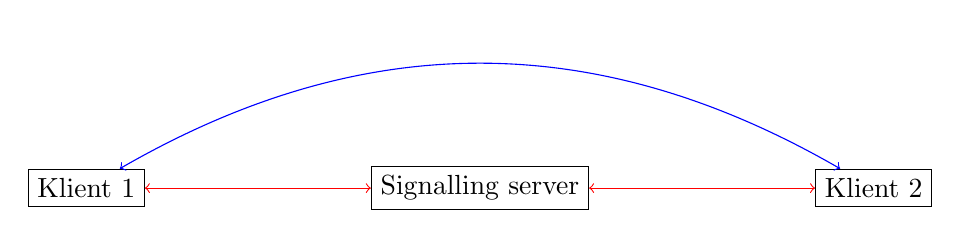
\begin{tikzpicture}
        \node[draw] (server) at (0,0) {Signalling server};
        \node[draw] (client1) at (-5, 0) {Klient 1};
        \node[draw] (client2) at (5, 0) {Klient 2};

        \draw[red, <->] (server) -- (client1);
        \draw[red, <->] (server) -- (client2);
        \draw[blue, <->] (client1) edge[bend left=30] (client2);
    \end{tikzpicture}
    \caption{Signalling}
    \label{signallingServer}
\end{figure}

\textit{Signalling} je zásadní součást \gls{webrtc}. Jedná se o proces při
kterém si klienti vyměňují pomocí tzv. \textit{signalling serveru} \gls{ice}
kandidáty a informace o tom, jaká data plánují posílat, jaké
kodeky\footnote{Kodek je hardware či software, který se využívá pro zakódování,
    či rozkódování médii \parencite{Britannica-Codec,TechTarget-Codec}.} podporují
atp. Zprávy, které si klienti pomocí signalling serveru vyměňují, se nazývají
\textit{session descriptions}. Jsou ve formátu, který je definován protokolem
zvaným \gls{sdp} (místo \textit{session description} se někdy píše jen
\gls{sdp})~\parencite{WebRTCForTheCurious}. Signalling server není nijak
standardizován, jedinou podmínkou je, že realizuje výměnu \gls{sdp}. To vede k
tomu, že aplikace často nejsou mezi sebou kompatibilní
\parencite{MDN-Web-SignalingAndVideoCalling}.

Chce-li klient 1 volat klienta 2, vygeneruje tzv. \textit{session description
    offer} (\textit{\gls{sdp} offer}), kterou pomocí signalling serveru přepošle
klientovi 2. Chce-li klient 2 hovor přijmout, vygeneruje tzv.
\textit{session description answer} (\textit{\gls{sdp} answer}), kterou
naopak přepošle klientovi~1. Poté, co dojde k výměně session descriptions,
se protokol \gls{ice} pokusí vybrat vhodný pár kandidátů. Tento proces se
nazývá \textit{negotiation}
\parencite{WebRTCForTheCurious,MozillaBlog-PerfectNegotiation}.

Dojde-li během hovoru ke změnám spojení (změní se stopy, které klienti posílají,
či se změní pozice klienta na síti), proběhne tzv. \textit{renegotiation}, kdy
se proces výměny session descriptions opakuje
\parencite{MozillaBlog-PerfectNegotiation}.

\gls{sdp} se skládá z \textit{párů klíč-hodnota} (\textit{key-value pairs}).
Každý pár má následující formát: \mintinline{text}{<klíč>=<hodnota>}. \gls{sdp}
může stejný klíč obsahovat několikrát. \parencite{WebRTCForTheCurious}. Je-li
hodnota nedefinovaná, používá se znak \mintinline{text}{-}
\parencite{IETF-RFC8866}. Záleží na pořadí jednotlivých řádků -- \gls{sdp}
začíná obecnými informacemi o spojení, které jsou následovány jednotlivými
média-sekcemi. Média-sekce popisuje jednu odchozí stopu a jednu příchozí stopu
(obě stopy nemusí být nutně aktivní), které musí být stejného typu (audio, anebo
video). \gls{sdp} podporuje několik klíčů, \gls{webrtc} využívá následující
\parencite{WebRTCForTheCurious,IETF-RFC8866}:

\begin{itemize}
    \item \mintinline{text}{v} -- značí verzi, která je vždy
          \mintinline{text}{0}
    \item \mintinline{text}{o} -- popisuje tvůrce spojení, slouží jako jeho
          unikátní identifikátor, skládá se z:
          \begin{itemize}
              \item \mintinline{text}{username} -- ID uživatele, který zahájil
                    spojení
              \item \mintinline{text}{sess-id} -- unikátní číslo, které
                    identifikuje spojení
              \item \mintinline{text}{sess-version} -- verze session
                    description, která by se měla po každé změně zvýšit
              \item \mintinline{text}{nettype} -- typ sítě, je vždy
                    \mintinline{text}{IN} (internet)
              \item \mintinline{text}{addrtype} -- typ adresy, je buď
                    \mintinline{text}{IP4}, nebo \mintinline{text}{IP6}
              \item \mintinline{text}{unicast-address} -- IP adresa tvůrce
                    spojení
          \end{itemize}
    \item \mintinline{text}{s} -- název session, \gls{sdp} nesmí obsahovat více
          než jeden klíč \mintinline{text}{s}
    \item \mintinline{text}{c} -- informace o spojení, pro \gls{webrtc} není
          klíč \mintinline{text}{c} příliš zásadní, neboť se pro spojování
          využívá protokolu \gls{ice} (více v části \ref{connecting}), skládá se
          z:
          \begin{itemize}
              \item \mintinline{text}{nettype} -- typ sítě, je vždy
                    \mintinline{text}{IN} (internet)
              \item \mintinline{text}{addrtype} -- typ adresy, je buď
                    \mintinline{text}{IP4}, nebo \mintinline{text}{IP6}
              \item \mintinline{text}{connection-address} -- IP adresa využita
                    ke spojení
          \end{itemize}
    \item klíč \mintinline{text}{t} -- čas, kdy spojení začíná a končí, skládá
          se z:
          \begin{itemize}
              \item \mintinline{text}{start-time} -- čas, kdy spojení začne;
                    pokud je \mintinline{text}{0}, spojení je permanentní
              \item \mintinline{text}{stop-time} -- čas, kdy spojení skončí;
                    pokud je \mintinline{text}{0}, doba spojení není omezena
          \end{itemize}
    \item \mintinline{text}{a} -- atribut, jeho formát je
          \mintinline{text}{a=<jméno>:<hodnota>}; \gls{sdp} může obsahovat
          několik klíčů \mintinline{text}{a}, ať už pro celé spojení, nebo pro
          specifickou média-sekci
    \item \mintinline{text}{m} -- popis médií, skládá se z:
          \begin{itemize}
              \item \mintinline{text}{media} -- typ média, je buď
                    \mintinline{text}{audio}, \mintinline{text}{video},
                    \mintinline{text}{application}, \mintinline{text}{text},
                    nebo \mintinline{text}{message}
              \item \mintinline{text}{port} -- port, který je využit k posílání
                    dat
              \item \mintinline{text}{proto} -- protokol, hodnoty mohou být:
                    \begin{itemize}
                        \item \mintinline{text}{udp} -- data jsou posílána přímo
                              přes protokol \gls{udp}
                        \item \mintinline{text}{RTP/AVP} -- data jsou posílána
                              pomocí protokolu RTP (více v části \ref{rtp})
                              s~profilem pro audio a video
                        \item \mintinline{text}{RTP/SAVP} -- data jsou posílána
                              pomocí protokolu \gls{srtp} (více v části
                              \ref{srtp})
                        \item \mintinline{text}{RTP/SAVPF} -- data jsou posílána
                              pomocí protokolu \gls{srtp} s podporou pro
                              \gls{rtcp} (více v části \ref{rtcp})
                    \end{itemize}
              \item \mintinline{text}{fmt} -- seznam čísel, která určují
                    podporované formáty dat; čísla od \mintinline{text}{0} do
                    \mintinline{text}{95} referují ke specifickým formátům; u
                    čísel od \mintinline{text}{96} do \mintinline{text}{127} se
                    využívá atributu \mintinline{text}{a=rtpmap:<fmt> <codec>}
                    pro specifikaci kodeku
          \end{itemize}
\end{itemize}

\gls{sdp} podporuje několik různých atributů, ty následující jsou zásadní pro
fungování \gls{webrtc}
\parencite{WebRTCForTheCurious,IETF-RFC8866,IETF-RFC5888,IETF-RFC8841}:
\begin{itemize}
    \item \mintinline{text}{a=group:BUNDLE} značí, že přes jedno peer spojení
          posíláme více stop; některé implementace vytváří jedno peer spojení na
          každou stopu, což ale není doporučeno
    \item \mintinline{text}{a=sendrecv}, \mintinline{text}{a=sendonly},
          \mintinline{text}{a=recvonly} a \mintinline{text}{a=inactive} --
          značí, směr dat dané média-sekce; oba klienti by se měli shodnout na
          směru dat, obsahuje-li tedy \gls{sdp} offer
          \mintinline{text}{a=sendonly}, \gls{sdp} answer by měla obsahovat
          \mintinline{text}{a=recvonly} pro danou média-sekci
    \item \mintinline{text}{a=mid} -- číslo média-sekce
    \item \mintinline{text}{a=msid} -- ID stopy a streamu, má formát
          \mintinline{text}{<ID streamu> <ID stopy>}
    \item \mintinline{text}{a=rtpmap} -- zmíněno v předchozím odstavci
    \item \mintinline{text}{a=sctp-port} -- port používaný protokolem \gls{sctp}
          (více v části \ref{sctp})
    \item \mintinline{text}{a=max-message-size} -- maximální velikost zprávy v
          bytech
\end{itemize}

\gls{sdp} zároveň podporuje několik atributů, které se využívají pro nastavení
\gls{ice} a výměnu \gls{ice} kandidátů
\parencite{WebRTCForTheCurious,IETF-RFC8839}:
\begin{itemize}
    \item \mintinline{text}{a=ice-ufrag} -- uživatelské jméno, používáno pro
          ověření integrity
    \item \mintinline{text}{a=ice-pwd} -- heslo, používáno pro ověření integrity
    \item \mintinline{text}{a=ice-options} -- specifikuje rozšíření, které
          klient podporuje
    \item \mintinline{text}{a=candidate} -- je na úrovni média-sekce a
          specifikuje informace o daném \gls{ice} kandidátu
\end{itemize}

Níže můžeme vidět příklad reálného \gls{sdp}, které obsahuje 3 média-sekce. Obě
používají port \mintinline{text}{4000} a protokol \mintinline{text}{RTP/AVP}. V
klíči \mintinline{text}{o} je důležité třetí pole s hodnotou
\mintinline{text}{2}, která indikuje verzi session description. Klíč
\mintinline{text}{s} nemá hodnotu, spojení je tedy bez názvu. Klíč
\mintinline{text}{c} je pak pro \gls{webrtc} nepodstatný.

\begin{figure}[H]
    \begin{minted}[breaklines,fontsize=\footnotesize]{text}
v=0
o=- 2021867665009852994 2 IN IP4 127.0.0.1
s=-
c=IN IP4 192.168.1.1
t=0 0
a=group:BUNDLE 0 1
a=ice-ufrag:o6S/
a=ice-pwd:mXxyUi9PVAiuCPvl
a=ice-options:trickle
m=audio 4000 RTP/AVP 0 111
a=mid:0
a=sendrecv
a=candidate:foundation 1 udp 2130706431 192.168.1.1 53165 typ host generation 0
a=end-of-candidates
a=msid:yvKPspsHcYcwGFTw DfQnKjQQuweLFdV
a=rtpmap:111 OPUS/48000/2
m=video 4000 RTP/AVP 96
a=mid:1
a=sendonly
a=msid:yvKPspsHcYcwGFTw Ii65zvjKITaFf0T
a=rtpmap:96 VP8/90000
m=application 9 UDP/DTLS/SCTP webrtc-datachannel
a=mid:2
a=sctp-port:5000
a=max-message-size:262144
    \end{minted}
\end{figure}

První sekce je \mintinline{text}{audio}, její \mintinline{text}{mid} je
\mintinline{text}{0} a její směr je \mintinline{text}{sendrecv}, takže umožňuje
přijímání i~posílání audio stopy. Formát je dynamický a z
\mintinline{text}{a=rtpmap} je vidět, že~\mintinline{text}{111} označuje kodek
Opus. Můžeme si rovněž povšimnout specifikace ID streamu a stopy.

Druhá sekce je \mintinline{text}{video}, její \mintinline{text}{mid} je
\mintinline{text}{1} a její směr je \mintinline{text}{sendonly}, klient tedy
může používat tuto média-sekci pro posílání videa. Formát je opět dynamický, z
\mintinline{text}{a=rtpmap} je vidět, že~číslo \mintinline{text}{96} označuje
kodek VP8. Je také vidět, že stopa patří do stejného streamu jako stopa v první
média-sekci.

Třetí sekce je \mintinline{text}{application} a popisuje datový kanál. Její
\mintinline{text}{mid} je \mintinline{text}{2}. Protokol \gls{sctp} využívá port
\mintinline{text}{5000} a maximální velikost zprávy je \mintinline{text}{262144}
\si{\byte}, což je \mintinline{text}{256} \si{\kibi\byte}.

Další klíče se týkají protokolu \gls{ice}, který je popsán v části \ref{ice}.
